% Mestre em LaTeX - v0.5
% Copyleft 2008-2013 Bruno C. Vellutini - http://organelas.com/
%
% Permission is hereby granted, free of charge, to any person obtaining a copy
% of this software and associated documentation files (the "Software"), to deal
% in the Software without restriction, including without limitation the rights
% to use, copy, modify, merge, publish, distribute, sublicense, and/or sell
% copies of the Software, and to permit persons to whom the Software is
% furnished to do so, subject to the following conditions:
%
% THE SOFTWARE IS PROVIDED "AS IS", WITHOUT WARRANTY OF ANY KIND, EXPRESS OR
% IMPLIED, INCLUDING BUT NOT LIMITED TO THE WARRANTIES OF MERCHANTABILITY,
% FITNESS FOR A PARTICULAR PURPOSE AND NONINFRINGEMENT. IN NO EVENT SHALL THE
% AUTHORS OR COPYRIGHT HOLDERS BE LIABLE FOR ANY CLAIM, DAMAGES OR OTHER
% LIABILITY, WHETHER IN AN ACTION OF CONTRACT, TORT OR OTHERWISE, ARISING FROM,
% OUT OF OR IN CONNECTION WITH THE SOFTWARE OR THE USE OR OTHER DEALINGS IN
% THE SOFTWARE.
%
% Ou seja, utilize e modifique os arquivos como desejar.
% 
% Para mais informações visite http://nelas.github.com/mestre-em-latex/

% Classe do documento
\documentclass[twoside,a4paper,11pt]{report}

% Pacotes e comandos customizados
%%% Pacotes utilizados %%%

%% Codificação e formatação básica do LaTeX
% Suporte para português (hifenação e caracteres especiais)
\usepackage[english,brazilian]{babel}

% Codificação do arquivo
\usepackage[utf8]{inputenx}

% Mapear caracteres especiais no PDF
\usepackage{cmap} 

% Codificação da fonte
\usepackage[T1]{fontenc}
% Usa a lmodern por padrão (caso cm-super não esteja instalada).
\usepackage{lmodern}

%% Microtipografia
% Utiliza recursos como espaçamento entre letras e entre linhas
\usepackage{microtype}
% Habilita protrusão e expansão, ignorando
% compatibilidade (ver documentação do pacote)
\microtypesetup{activate={true,nocompatibility}}
% factor=1100 aumenta a protrusão (default 1000)
% stretch=10 diminui o valor máximo de expansão (default 20)
% shrink=10 diminui o valor máximo de encolhimento (default 20)
\microtypesetup{factor=1100, stretch=10, shrink=10}
% Tracking, espaçamento entre palavras, kerning
\microtypesetup{tracking=true, spacing=true, kerning=true}
% Remover tracking para Small Caps
\SetTracking{encoding={T1}, shape=sc}{0}
% Remove ligaduras para o 'f'. Se necessário, adicionar letras
% separadas por vírgulas
\DisableLigatures[f]{encoding={T1}}
% Documento em versão "final", suporte para outros idiomas
\microtypesetup{final, babel}

% Essencial para colocar funções e outros símbolos matemáticos
\usepackage{amsmath,amssymb,amsfonts,textcomp}

%% Layout
% Customização do layout da página, margens espelhadas
\usepackage[twoside]{geometry}
% Aumenta as margens internas para espiral
\geometry{bindingoffset=10pt}
% Só pra ajustar o layout
\setlength{\marginparwidth}{90pt}
%\usepackage{layout}

% Para definir espaçamento entre as linhas
\usepackage{setspace} 

% Espaçamento do texto para o frame
\setlength{\fboxsep}{1em}

% Faz com que as margens tenham o mesmo tamanho horizontalmente
%\geometry{hcentering}

%% Elementos Gráficos
% Para incluir figuras (pacote extendido)
\usepackage[]{graphicx} 

%% Suporte a cores
\usepackage{color}
% Os argumentos declaram nomes novos, como Cyan e Crimson
% (ver documentação do pacote).
\usepackage[usenames,dvipsnames,svgnames]{xcolor}

% Criar figura dividida em subfiguras
\usepackage{subfig}
\captionsetup[subfigure]{style=default, margin=0pt, parskip=0pt, hangindent=0pt, indention=0pt, singlelinecheck=true, labelformat=parens, labelsep=space}

% Caso queira guardar as figuras em uma pasta separada
% (descomente e) defina o caminho para o diretório:
%\graphicspath{{./figuras/}}

% Customizar as legendas de figuras e tabelas
\usepackage{caption}

% Criar ambientes com 2 ou mais colunas
\usepackage{multicol}

% Ative o comando abaixo se quiser colocar figuras de fundo (e.g., capa)
%\usepackage{wallpaper}
% Exemplo para inserir a figura na capa está no arquivo pre.tex (linha 7)
% Ajuste da posição da figura no eixo Y
%\addtolength{\wpYoffset}{-140pt}
% Ajuste da posição da figura no eixo X
%\addtolength{\wpXoffset}{36pt}

%% Tabelas
% Elementos extras para formatação de tabelas
\usepackage{array}

% Tabelas com qualidade de publicação
\usepackage{booktabs}

% Para criar tabelas maiores que uma página
\usepackage{longtable}

% adicionar tabelas e figuras como landscape
\usepackage{lscape}

%% Lista de Abreviações
% Cria lista de abreviações
\usepackage[notintoc,portuguese]{nomencl}
\makenomenclature

%% Notas de rodapé
% Lidar com notas de rodapé em diversas situações
\usepackage{footnote}

% Notas criadas nas tabelas ficam no fim das tabelas
\makesavenoteenv{tabular}

% Conta o número de páginas
\usepackage{lastpage}

%% Referências bibliográficas e afins
% Formatar as citações no texto e a lista de referências
%\usepackage{natbib}
\usepackage[authoryear,round,longnamesfirst]{natbib}
% Adicionar bibliografia, índice e conteúdo na Tabela de conteúdo
% Não inclui lista de tabelas e figuras no índice
\usepackage[nottoc,notlof,notlot]{tocbibind}

%% Pontuação e unidades
% Posicionar inteligentemente a vírgula como separador decimal
\usepackage{icomma}

% Formatar as unidades com as distâncias corretas
\usepackage[tight]{units}

%% Cabeçalho e rodapé
% Controlar os cabeçalhos e rodapés
\usepackage{fancyhdr}
% Usar os estilos do pacote fancyhdr
\pagestyle{fancy}
\fancypagestyle{plain}{\fancyhf{}}
% Limpar os campos do cabeçalho atual
\fancyhead{}
% Número da página do lado esquerdo [L] nas páginas ímpares [O] e do lado direito [R] nas páginas pares [E]
\fancyhead[LO,RE]{\thepage}
% Nome da seção do lado direito em páginas ímpares
\fancyhead[RO]{\nouppercase{\rightmark}}
% Nome do capítulo do lado esquerdo em páginas pares
\fancyhead[LE]{\nouppercase{\leftmark}}
% Limpar os campos do rodapé
\fancyfoot{}
% Omitir linha de separação entre cabeçalho e conteúdo
\renewcommand{\headrulewidth}{0pt}
% Omitir linha de separação entre rodapé e conteúdo
\renewcommand{\footrulewidth}{0pt}
% Altura do cabeçalho
\headheight 15pt

% Dados do projeto
\newcommand{\nomedoaluno}{Hudson Chaves Costa}
\newcommand{\titulo}{Três Ensaios em Comportamento dos Preços na Economia Brasileira}

%% Links dinâmicos
% Suporte para hipertexto, links para referências e figuras
\usepackage{hyperref}
% Configurações dos links e metatags do PDF a ser gerado
\hypersetup{colorlinks=true, linkcolor=blue, citecolor=blue, filecolor=blue, pagecolor=blue, urlcolor=green,
            pdfauthor={\nomedoaluno},
            pdftitle={\titulo},
            pdfsubject={Assunto do Projeto},
            pdfkeywords={palavra-chave, palavra-chave, palavra-chave},
            pdfproducer={LaTeX},
            pdfcreator={pdfTeX}}

%% Inserir comentários no texto
% Marcar mudanças e fazer comentários
%\usepackage[margins]{trackchanges}
% Iniciais do autor
%\renewcommand{\initialsTwo}{bcv}
% Notas na margem interna
%\reversemarginpar

%% Comandos customizados

% Espécie e abreviação
\newcommand{\subde}{\emph{Clypeaster subdepressus}}
\newcommand{\subsus}{\emph{C.~subdepressus}}

%% Pacotes não implementados
% Para não sobrar espaços em branco estranhos
%\widowpenalty=1000
%\clubpenalty=1000
\usepackage{listings}

% Início do texto
\usepackage{Sweave}
\begin{document}
\Sconcordance{concordance:ensaio01.tex:ensaio01.Rnw:%
1 25 1}
\Sconcordance{concordance:ensaio01.tex:./metaen01.Rnw:ofs 26:%
1 190 1}
\Sconcordance{concordance:ensaio01.tex:ensaio01.Rnw:ofs 217:%
28 2 1 1 0 2 1}
\Sconcordance{concordance:ensaio01.tex:./preen01.Rnw:ofs 223:%
1 217 1}
\Sconcordance{concordance:ensaio01.tex:./cap1en01.Rnw:ofs 441:%
1 66 1}
\Sconcordance{concordance:ensaio01.tex:./cap2en01.Rnw:ofs 508:%
1 98 1}
\Sconcordance{concordance:ensaio01.tex:./cap3en01.Rnw:ofs 607:%
1 187 1}
\Sconcordance{concordance:ensaio01.tex:ensaio01.Rnw:ofs 795:%
37 14 1}


% Limpa cabeçalhos.
% (solução para lidar com a númeração das páginas pré-textuais).
\pagestyle{empty}

%% Capa
\begin{titlepage}

% Se quiser uma figura de fundo na capa ative o pacote wallpaper
% e descomente a linha abaixo.
% \ThisCenterWallPaper{0.8}{nomedafigura}

\begin{center}
{\LARGE \nomedoaluno}
\par
\vspace{200pt}
{\Huge \titulo}
\par
\vfill
\textbf{{\large Porto Alegre}\\
{\large \the\year}}
\end{center}
\end{titlepage}

% Faz com que a página seguinte sempre seja ímpar (insere pg em branco)
\cleardoublepage

% Numeração em elementos pré-textuais é opcional (ativada por padrão).
% Para desativá-la comente a linha abaixo.
%\pagestyle{fancy}

% Números das páginas em algarismos romanos
\pagenumbering{roman}

%% Página de Rosto

% Numeração não deve aparecer na página de rosto.
\thispagestyle{empty}

\begin{center}
{\LARGE \nomedoaluno}
\par
\vspace{200pt}
{\Huge \titulo}
\end{center}
\par
\vspace{90pt}
\hspace*{175pt}\parbox{7.6cm}{{\large Projeto de Tese apresentado ao Programa de Pós-Graduação em Economia da Universidade Federal do Rio Grande do Sul na Área de Economia Aplicada.}}

\par
\vspace{1em}
\hspace*{175pt}\parbox{7.6cm}{{\large Orientador: Prof. Dr. Sabino Porto da Silva Júnior}}

\par
\vfill
\begin{center}
\textbf{{\large Porto Alegre}\\
{\large \the\year}}
\end{center}

\newpage

% Ficha Catalográfica
%\hspace{8em}\fbox{\begin{minipage}{10cm}
%Aluno, Nome C.

%\hspace{2em}\titulo

%\hspace{2em}\pageref{LastPage} páginas

%\hspace{2em}Dissertação (Mestrado) - Instituto de Biociências da Universidade de São Paulo. Departamento de XXXXXXXX.

%\begin{enumerate}
%\item Palavra-chave
%\item Palavra-chave
%\item Palavra-chave
%\end{enumerate}
%I. Universidade de São Paulo. Instituto de Biociências. Departamento de XXXXXXXX.

%\end{minipage}}
%\par
%\vspace{2em}
%\begin{center}
%{\LARGE\textbf{Comissão Julgadora:}}

%\par
%\vspace{10em}
%\begin{tabular*}{\textwidth}{@{\extracolsep{\fill}}l l}
%\rule{16em}{1px}   & \rule{16em}{1px} \\
%Prof. Dr.   	& Prof. Dr. \\
%Nome			& Nome
%\end{tabular*}

%\par
%\vspace{10em}

%\parbox{16em}{\rule{16em}{1px} \\
%Prof. Dr. \\
%Nome do Orientador}
%\end{center}

%\newpage

% Dedicatória
% Posição do texto na página
%\vspace*{0.75\textheight}
%\begin{flushright}
  %\emph{Dedicatória...}
%\end{flushright}

%\newpage

% Epígrafe
%\vspace*{0.4\textheight}
%\noindent{\LARGE\textbf{Exemplo de epígrafe}}
% Tudo que você escreve no verbatim é renderizado literalmente (comandos não são interpretados e os espaços são respeitados)
%\begin{verbatim}
%O que é bonito?
%É o que persegue o infinito;
%Mas eu não sou
%Eu não sou, não…
%Eu gosto é do inacabado,
%O imperfeito, o estragado, o que dançou
%O que dançou…
%Eu quero mais erosão
%Menos granito.
%Namorar o zero e o não,
%Escrever tudo o que desprezo
%E desprezar tudo o que acredito.
%Eu não quero a gravação, não,
%Eu quero o grito.
%Que a gente vai, a gente vai
%E fica a obra,
%Mas eu persigo o que falta
%Não o que sobra.
%Eu quero tudo que dá e passa.
%Quero tudo que se despe,
%Se despede, e despedaça.
%O que é bonito…
%\end{verbatim}
%\begin{flushright}
%Lenine e Bráulio Tavares
%\end{flushright}

%\newpage

% Agradecimentos

% Espaçamento duplo
%\doublespacing

%\noindent{\LARGE\textbf{Agradecimentos}}

%Agradeço ao meu orientador, ao meu co-orientador, aos meus colaboradores, aos técnicos, à seção administrativa, à fundação que liberou verba para minhas pesquisas, aos meus amigos, à minha família e ao meu grande amor.

%\newpage

%\vspace*{10pt}
% Abstract
%\begin{center}
  %\emph{\begin{large}Resumo\end{large}}\label{resumo}
%\vspace{2pt}
%\end{center}
% Pode parecer estranho, mas colocar uma frase por linha ajuda a organizar e reescrever o texto quando necessário.
% Além disso, ajuda se você estiver comparando versões diferentes do mesmo texto.
% Para separar parágrafos utilize uma linha em branco.
%\noindent
%Esta, quem sabe, é a parte mais importante do seu trabalho.
%É o que a maioria das pessoas vai ler (além do título).
%Seja objetivo sem perder conteúdo.
%Um bom resumo explica porquê este trabalho é interessante, relata como foi feito, o que foi encontrado, contextualiza os resultados e delineia conclusões.
%\par
%\vspace{1em}
%\noindent\textbf{Palavras-chave:} palavra1, palavra2, palavra3
%\newpage

% Criei a página do abstract na mão, por isso tem bem mais comandos do que o resumo acima, apesar de serem idênticas.
%\vspace*{10pt}
% Abstract
%\begin{center}
  %\emph{\begin{large}Abstract\end{large}}\label{abstract}
%\vspace{2pt}
%\end{center}

% Selecionar a linguagem acerta os padrões de hifenação diferentes entre inglês e português.
%\selectlanguage{english}
%\noindent
%This is the most important part of your work.
%This is what most people will read.
%Be concise without omitting content.
%A good abstract explains why this is an interesting study, tells how it was done, what was found, contextualizes the results and set conclusions.
%\par
%\vspace{1em}
%\noindent\textbf{Keywords:} word1, word2, word3

% Voltando ao português...
%\selectlanguage{brazilian}

%\newpage

% Desabilitar protrusão para listas e índice
\microtypesetup{protrusion=false}

% Lista de figuras
%\listoffigures

% Lista de tabelas
%\listoftables

% Abreviações
% Para imprimir as abreviações siga as instruções em 
% http://code.google.com/p/mestre-em-latex/wiki/ListaDeAbreviaturas
%\printnomenclature

% Índice
\tableofcontents

% Re-habilita protrusão novamente
\microtypesetup{protrusion=true}
% Faz com que o ínicio do capítulo sempre seja uma página ímpar
\cleardoublepage

% Inclui o cabeçalho definido no meta.tex
\pagestyle{fancy}

% Números das páginas em arábicos
\pagenumbering{arabic}

\chapter{INTRODUÇÃO/MOTIVAÇÃO}\label{intro}

% É sabido da importância dos preços para a alocação de recursos, dado que na ocorrência de rigidez de preços, a alocação ineficiente é uma consequência. O grau da rigidez para diferentes produtos alinhado a uma política monetária expansionista impactarão os preços relativos que por sua vez influenciarão a economia real. O estudo da rigidez de preços é tema importante para a avaliação do comportamento da inflação que permite analisar o grau de persistência inflacionária e assim, melhor uso dos instrumentos de política monetária. Em resposta à relevância do tema, modelos macroeconômicos de preços rígidos têm sido desenvolvidos e fundamentam-se, em grande medida, no comportamento microeconômico de determinação de preços adotado pelos agentes. 

% Ainda, muito da macroeconomia se baseia em alguma fonte de rigidez para gerar desempenho ineficiente.
% Além disso, estudar a rigidez de preços é fundamental para a análise do comportamento da inflação

% Não obstante, sabemos que os preços geralmente são considerados rígidos ou lentos para se ajustarem, pois a presença de algum tipo de restrição, frequentemente denominada de rigidez nominal, implica em dificuldade de ajustamento instantâneo ou sem qualquer custo. Diversos modelos econômicos incluem mecanismos para incorporar essa rigidez nominal. Além disso, um número de diferentes mecanismos tem sido propostos e podem ser divididos em dois principais grupos: preços tempo-dependentes e estado-dependentes

% Examinar como os preços se comportam pode ajudar a identificar qual destes modelos teóricos são mais relevantes para a economia real. 
% Assim, conhecer mais sobre quão frequentemente os preços indivíduais mudam e a magnitute das variações é essencial para os toamdores de decisões e ponto de partica para modeloes microfundamentados.

% Na maneira mais simples do modelo proposto por \citet{calvo1983staggered}, firmas homogêneas têm uma probabilidade fixa de mudar seus preços em cada período (isto é, a probabilidade de um preço mudar não depende de quando a alteração anterior ocorreu). Modelos tempo-dependentes alternativos salientam que os preços são fixos em função da existência de contratos que se sobrepõem dado que eles não começam e finalizam ao mesmo tempo (\citet{taylor1980aggregate}).

% A partir disso, este ensaio do projeto de tese, busca aplicar a teconologia de \emph{web scraping} na avaliação de como os preços individuais ao consumidor tipicamente se comportam e se existe rigidez de preços nos principais mercados brasileiros\footnote{A princípio serão coletados preços dos principais sites das regiões metropolitanas e cidades que participam do IPCA e INPC}. Isto permitirá uma períodicidade diária na coleta de preços e maior quantidade de preços coletados em comparação com os tradicionais índices de preços.  

% Pretende-se contribuir para o estudo empírico da rigidez nominal nos preços por meio da estimação de funções de risco de alterações nos preços. Esta função é definida como a probabilidade condicional dos preços se alterarem em relação ao tempo, um conceito chave em entender o comportamento dos preços. Ela está relacionada aos modelos microfundamentados. Por exemplo, os modelos de \citet{calvo1983staggered} e \citet{taylor1980aggregate} têm função de risco constante. A probabilidade de alterações nos preços depende apenas do tempo, independentemente de mudanças em variáveis de estado. Por outro lado, o modelo de \citet{dotsey1999state} tem uma função de risco crescente que muda dependendo das variáveis de estado. Ele é um dos mais populares modelos estado-dependentes em um framework de equilibrio geral. 

Firmas individuais não ajustam seus preços em contrapartida de choques relevantes na economia. Este fato não é controvérsia e é uma hipótese padrão em modelagem macroeconômica que permite choques nominais influenciar as variáveis reais. Uma grande vertente da literatura analisou as implicações de alternativas formas de rigidez nominal sobre a dinâmica do comportamento da inflação e produto em níveis agregados. Não obstante, em resposta à relevância do tema, modelos macroeconômicos de preços rígidos têm sido desenvolvidos e fundamentam-se, em grande medida, no comportamento microeconômico de determinação de preços adotado pelos agentes. 

Os diferentes mecanismos propostos para incorporar a rigidez nominal dos preços podem ser divididos em dois grupos: preços tempo-dependentes e preços estado-dependentes. Em um modelo de precificação tempo-dependente, a possibilidade de um preço mudar pode ser afetada apenas pelo tempo desde a mudança anterior e não pelo estado das vendas de uma firma, a economia ou outros fatores. Já em modelos estado-dependentes, a decisão de mudar os preços depende do estado da economia e o mercado enfrentado pela firma. Firmas enfrentam custos caso ajustem seus preços e exemplos destes custos incluem custos fixos (custo de menu, \citet{mankiw1985small}) ou a desutilidade associada à fazer grandes alteraçõeses de preços se as firmas temem que tais mudanças podem contrariar seus clientes (\citet{rotemberg1982sticky}). 

Na mesma direção da preocução teórica em relação ao comportamento dos preços, muitos Bancos Centrais têm adotado a política de metas de inflação como um fator relevante para a política monetária. Tipicamente, a meta é definida em termos de um índice de preço agregado, tal como o Índice Nacional de Preços ao Consumidor Amplo (IPCA) no Brasil. Dado que este índice agregado é uma soma ponderada dos preços individuais, mudanças nestes preços terão importantes implicações para o nível de preço geral e preços relativos. A partir disso, foi natural o surgimento de pesquisas com o objetivode diferir a análise empírica da rigidez nominal dos preços baseada em dados agregados da avaliação do comportamento dos preços por meio de microfundamentos. 

Por conseguinte, recentes estudos têm usado de grandes bancos de dados de preços individuais (microdados) para examinar como os preços ao consumidor comportam em nível de produto. Em particular, \citet{bils2004some}, \citet{nakamura2008five} e \citet{klenow2008state} para os EUA, \citet{dhyne2006price} para a Zona do Euro, \citet{gouvea2007nominal}, \citet{matos2009comportamento} e \citet{lopes2008rigidez} para o Brasil e \citet{bunn2012examining} para o Reino Unido. Apesar de pesquisas brasileiras terem utilizado de microdados para a avaliação empirica da rigidez dos preços, nenhuma delas conseguiu alta granularidade no que tange à periodicidade dos preços coletados bem como em relação às regiões em que a rigidez foi avaliada. Tal característica é oriunda da fontes de dados usadas (IBRE/FGV e IPC/FIPE). 

Assim, pesquisas anteriores têm demonstrado a importância da avaliação da rigidez nominal dos preços usando microdados. Os fatos estilizados obtidos de microdados podem ajudar a examinar o comportamento dos preços em nível de firmas, onde as decisções de precificação são feitas. A informação individual sobre as definições de preços permite determinar em que medida as hipóteses usadas na derivação de modelos teóricos são atualmente realísticas, o que por sua vez refina as estratégias de modelagem. Motivado por tais apontamentos, o presente ensaio explorará preços coletados de sites (supermercados, farmácias, lojas de eletrodomésticos, construção civil, ....) como uma alternativa à dificuldade em obter microdados de preços. A teconologia de \emph{web scraping} que será utilizada tem se tornado uma alternativa para o acesso a diversas fontes de dados para análise econômica empírica. 

Este ensaio é organizado da seguinte forma: além deste primeiro capítulo que faz uma breve apresentaçãoo do tema, justificativa e objetivos do ensaio, o capítulo 2 apresenta a revisão bibliográfica do tema e por fim no capítulo 3 a metodologia a ser utilizada bem como o cronograma da pesquisa são descritos.

\subsection*{JUSTIFICATIVA}

A dinâmica do comportamento dos preços individuais proporciona vários desdobramentos que são bastante debatidos na literatura dado os impactos que podem causar. Não compreender este tipo de comportamento levou a distintas abordagens para a análise da velocidade e intensidade de transmissão da política monetária. Além disso, compreender as estratégias de definição de preços das firmas levaria ao aprimoramento de modelos teóricos cujas abordagens e conclusões podem sofrer alterações expressivas na presença de fatos estilizados. 

A falta de estudos que gerassem empiricamente um diagnóstico da definição e grau de rigidez de preços individuais foi um limitador por diversas décadas em função da falta de informações estatísticas no nível de microdados que pudessem servir de base para estas análises. Porém, há alguns anos a disponibilização de preços coletados pelos órgãos governamentais tanto nacionais quanto internacionais, proporcionaram o surgimento de pesquisas que avaliassem o comportamento dos preços em nível de microdados (\citet{bils2004some,nakamura2008five,klenow2008state,dhyne2006price,gouvea2007nominal,matos2009comportamento,lopes2008rigidez,bunn2012examining}). 

Porém, ainda existe um fator limitante nestes estudos, pois concentram-se em mercados específicos, não possibilitando análises generalizadas aos diversos setores da economia, pois as pesquisas são reféns das características dos dados utilizados. Também, dada a importância do tema para os tomadores de decisão em nível de política monetária, é preciso maior dinâmica na análise e não apenas um olhar para o passado. 

Assim, o presente ensaio do projeto de tese apresenta o uso da tecnologia de \emph{web scraping} para coletar preços diretamente das páginas das empresas que possuem sites de vendas e por conseguinte, contribuir para a avaliação da rigidez de preços de uma forma mais dinâmica dadas as características do processo de coleta. Estudos empiricos já mostraram a importância de dados coletados da \emph{web} na avaliação dos pressupostos de rigidez de preços e proposição de medida de inflação oriunda de informações \emph{online} (\citet{cavallo2010scraped}).

\subsection*{OBJETIVOS}

O objetivo geral deste ensaio é avaliar empiricamente a rigidez nominal dos preços na economia brasileira por meio de dados coletados da \emph{web}, bem como, propor um índice de inflação oriundo da mesma fonte de dados que seja estatisticamente significante para o uso dos tomadores de decisões econômicas.

Dentro deste escopo, os seguintes questionamentos pretendem ser avaliados:

\begin{itemize}
  \item É possível utilizar os dados coletados da internet como proxy para a inflação divulgada pelos órgãos públicos?
  \item Quão frequente os preços se alteram?
  \item Existe heterogeneidade da rigidez nomial entre setores?
  \item Como podemos lidar com o problema de censura e amostragem quando a função risco é estimada a partir dos dados coletados da internet?
  \item A probabilidade de mudança dos preços pode variar ao longo da duração dos preços?
  \item Como podemos avaliar o efeito de variáveis explicativas sobre a taxa de risco?
\end{itemize}


\pagestyle{empty}
\cleardoublepage
\pagestyle{fancy}

\chapter{REVISÃO BIBLIOGRÁFICA}\label{cap2}

\section*{MODELOS DE PRECIFICAÇÃO}

Existem diversas abordagens teóricas na literatura de modelos de rigidez nominal em nível individual. Eles são baseados em várias hipóteses para os preços não se ajustarem: Contratos de Calvo/Taylor, Custo de Menu, Informação Rígida, Ira do Cliente. Na sequência, revisamos cada uma destas hipóteses e suas implicações para os modelos de precificação.

\subsection*{Contratos de Calvo/Taylor}

Preços nominais de acordo com \citet{taylor1980aggregate} são fixos por um certo número de períodos. Se as alterações nos preços fossem perfeitamente escalonados ao longo do tempo, a duração dos preços nominais permaneceriam constantes para todas as firmas. No modelo de Taylor, os preços são fixos por $N$ períodos e a taxa de risco é zero para todas as durações exceto $N$. 

No modelo de \citet{calvo1983staggered} a probabilidade de um preço mudar é constante. Em cada período, uma proporção fixa de firmas podem alterar seus preços, as firmas remanescentes mantêm seus preços nominais fixos. A probabilidade de ser capaz de mudar preços é a mesma para todas as firmas, independemente de quando elas mudaram seus preços pela última vez. Isto significa que a função risco é constante. 

Os modelos de Taylor e Calvo são insuficientes para gerar bastante persistência do produto e da inflação a choques de política monetária (Moore,1995;Chari et al., 2000; Christian et al., 2005) . 

Uma popular justificativa teórica é adicionar indexação ao modelo de Calvo (Smets e Wouters, 2003;Woodfor, 2003; Christiano et al., 2005). O preço é definido no começo do contrato e para a duração do contrato este é aumentado pela inflação do período. Embora seja possível o modelo de Calvo com indexação modelar a persistência da inflação e do produto, ele tem o custo de ter os preços alterando em todo o período. 

Os modelos de Taylo e Calvo generalizados são introduzidos para explicar a persistência da inflação e do produto sendo consistentes com a evidência micro de rigidez nominal. No modelo generalizado de Taylor, existem muitos setores com diferentes tamanho de preços e dentro de cada setor existem um simples processo de Taylor. No modelo generalizado de Calvo, a probabilidade de reposição é dependente da duração. Adicionalmente, podemos modelar a estratégia de definição dos preços como um modelo de Calvo com múltiplos setores, que é um caso especial do modelo generalizado de Calvo. Uma característica chave desses modelos generalizados é que eles refletem a grande heterogeneidade observada em dados individuais. A rigidez de preços varia entre setores. Na presença de complementariedade nos preços os setores de baixo ajuste tem um efeito maior e disproporcional sobre todos os ajustes de preços, retardando a resposta do preço e aumentando a resposta do produto a choques. Quando uma economia heterogênea é atingida por um choque, o ajustamento inicial ocorre principalmente em empresas de setores com ajuste rápido. Com o passar do tempo, uma grande proporção das firmas que ainda tem que ajustar são firmas de setores com ajustamento mais lento. Em outras palavras, o processo de ajuste é dominado inicialmente por ajustes de alta frequência e depois por ajustes de baixa frequência. 

Como proposto por Dixon (2012), pode-se relacionar o modelo generalizado de Taylor com dados individuais e olhar a distribuição cross-sectional da duração entre firmas e atrelar o modelo generalizado de Calvo através da função de risco. 

\subsection*{Custo de Menu}

Os modelos de custo de menu assumem que a mudança no preço é custosa e esse custo impede que as firmas mudem seus preços continuamente. Sheshinki e Weiss (1977) mostraram que na presença de custo de alteração nos preços, a política ótima de preços é a do tipo $(S,s)$. $S$ e $s$ indicam o limite superior e inferior para o preço real, respectivamente. Uma vez que o preço real encontra-se dentro dos limites, o preço nominal será mantido constante. Durante o período de precificação, a política ótima é um tipo de política estado-contingente.

Os modelos de custo de menu usualmente são resolvidos usando métodos numéricos, assim não há expressão analítica para a taxa de risco. Na maioria das calibrações realizadas por investigações anteriores, o risco é crescente com a duração.

\subsection*{Informção Rígida}

Assumem que é custoso para as firmas coletar informações sobre as condições econômicas correntes (Mankiw e Reis, 2002). Novas informações sobre o estado da economia tem sido adotadas e um novo padrão de preços ótimos são atualizadas em cada período. Informações desatualizadas são usadas para tomar decisões de preço pelo resto das empresas. A inflação, portanto, depende das expectativas anteriores da inflação e produto correntes.

Em função dos efeitos reais substancialmente maiores e persistentes serem resultados de choques monetários, o modelo de informação rígida ajusta fatores macroeconômicos melhores. Contudo, na ausência de outras fricções, alguma forma de indexação não importando se é geral, setorial ou em nível de preços, é envolvida no planejamento do preço ótimo das firmas. Portanto, todas as firmas mudam seus preços em todo o tempo em modelos de rigidez de informação. Este argumento, contudo, é contraditório nas evidências empíricas baseadas sobre dados individuais. Estudos anteriores fazem tentativas para resolver este problema por combinar rigidez de informação com custo de menu (klenow e Willis, 2006; Knotek, 2006). Uma economia em que as firmas se deparam tanto com custo de menu e o custo de conhecer as condições macroeconômicas precisa ser considerada. Dois métodos que as firmas podem adotar para obter informações é pagar os custos ou aprender as ações de outras empresas. Isto resulta em uma externalidade da informação e encoraja as firmas a atrasar o ajuste de preço.

\subsection*{Ira do Cliente}

Rotemberg (2005) desenvolveu um modelo para explicar a rigidez de preços. Este modelo indica que clientes sempre analisam as decisões de precificação das firmas dependendo da percepção de justiça. Se os clientes estão convictos que os preços não são justos, eles terão reações adversas para produtos ou serviços relevantes. Assim, firmas podem abandonar alterações nos preços para evitar a ira do cliente. 

Porém, consumidores não terão reação negativa e aceitam os ajustes de preços sobre as circuntâncias de rápida inflação. As empresas alterarão seus preços dentro de um calendário pertinente de forma que os clientes desenvolvam suas crenças.xvi 

\section*{PREÇOS RÍGIDOS E PREÇOS FLEXÍVEIS}

\citet{ball1994sticky} argumentam que a politica monetária afeta a atividade econômica real e que a principal razão para essa afirmação são as evidências históricas, especialmente os inúmeros episódios em que as contrações monetárias causaram recessões. Uma vez assumida a hipótese de não-neutralidade monetária, os macroeconomistas dividem-se quanto à melhor maneira de explicar flutuações econômicas de curto prazo. \citet{ball1994sticky} acreditam que a rigidez nominal dos preços fornece a explicação mais natural para a não-neutralidade monetária, dadas as evidências microeconômicas de que muitos preços são, de fato, rígidos. Outros economistas, entretanto, desenvolveram modelos com preços flexíveis e substituíram a rigidez nominal dos preços por alguma outra imperfeição nominal para geral o resultado de não-neutralidade monetária. 

A alternativa mais famosa aos modelos de preços rígidos é o moelo de \citet{lucas1972expectations}. Nesse modelo os preços são flexíveis e a imperfeição nominal é informacional, sendo possivel gerar o resultado de não-neutralidade monetária. O modelo de \citet{lucas1972expectations} de iformação imperfeita baseia-se na ideia de que quando um produtos observa uma mudança no preço de seu produto ele não sabe distinguir se isso é resultado de uma mudança no preço relativo ou se é resultado de uma mudança no nvel agregado de preços. Uma mudança nos preços relativos altera a quantidade ótima a produzir, enquanto que uma mudança no nível de preço agregado deixa a quantidade ótima de produção inalterada. Considerando-se uma expansão monetária não-observada, o melhor que cada produtor pode fazer é admitir que uma parte do aumento da demanda por seu produto reflete um choque de preços relativos. Então, produtores elevam seus produtos e a expansão monetária tem efeitos reais e não apenas efeitos nominais sobre os preços. A fragilidade do modelo de \citet{lucas1972expectations} esta no fato de que é difícil compreender como nas economias modernas produtores poderiam confundir movimentos nos preços relativos com movimentos no nível de preços agregado, dado o grande volume de informações. \citet{ball1994sticky} conclui que o modelo de Lucas não é um substituto convincente para os modelos de preços rígidos.

A vertente novo-keynesiana estabelece a hipótese de existência de rigidez nominal tanto nos preços quanto nos salários. Essas variáveis nominais teriam dificuldades em se ajustar dada a ocorrência de mudanças na política monetária o que, por conseguinte, provocaria impactos reais sobre o produto. Assim, a expansão monetária pode provocar diferentes impactos sobre cada preço da economia dependendo do grau de rigidez nominal de cada bem. Tal rigidez se for diversificada, resultará em alterações nos preços relativos provocando impactos reais.

Neste contexto, muitos modelos macroeconômicos de preços rígidos baseados em fundamentos microeconômicos têm sido desenvolvidos. As hipóteses desses modelos envolvem, em grande medida, características acerca do comportamento microeconômico de determinação de preços adotados pelos agentes. A busca da construção de modelos macroeconômicos cada vez mais apurados fez emergir a necessidade de verificar empiricamente alguns dos aspectos microeconômicos constantes nesses modelos. 

\section*{MODELOS TEMPO-DEPENDENTE E ESTADO-DEPENDENTE}

% Em modelos de rigidez de preços tempo-dependentes, o tempo de mudança no preço é exógeno. Em particular, uma firma pode definir seu preço $N$ períodos à frente (Fisher, 1977), apenas a cada $N$ períodos (\citet{taylor1980aggregate}) ou aleatoriamente (\citet{calvo1983staggered}). Os modelos de Taylor e Calvo apresentam escalonamento exógeno das variações de preços entre empresas na economia. Ou seja, os preços s?o reajustados de forma não coincidente. Como um resultado deste escalonamento, a fração de firmas ajustando seus preços é constante de período a período. Quando a demanda aumenta após uma expansão monetária, apenas uma fração de todos os preços aumentam e assim, o produto agregado real cresce. 
% 
% Modelos tempo-dependentes não têm fundamentos microeconômicos. Isto levou a a modelos de precificação estado-dependentes em que as empresas escolhem quando mudar seus preços sujeito à "custo de menu". As implicações desses modelos para o produto real e inflação podem diferir drasticamente dos modelos tempo-dependentes. Caplin e Spulber (1987), consideram um modelo de ajuste de preços endógeno em que, sobre certas hipóteses no processo monetário e distribuição dos preços, a moeda não tem efeito real, Subsequente pesquisa de Caballero e Engel (1993) e Caplin e Leahy (1991,1997) examinaram 
% 
% #################
% ### CONTINUAR AQUI COM O ARTIGO STATE-DEPENDENT OR TIME-DEPENDENT PRICING : DOES IT MATTER FOR RECENT U.S. INFLATION?
% #################

Em geral, modelos de precificação microfundamentados são classificados em dois tipos: modelos estado-dependentes e modelos tempo-dependentes. Nos modelos tempo-dependentes, a probabilidade dos preços mudarem depende apenas do período pelo qual o preço está fixo. Então, a função risco deste modelo tem uma certa forma constante em relação à duração dos preços. Por exemplo, o modelo \citet{calvo1983staggered} tem uma função de risco plana e assume que a oportunidade de um preço variar segue um processo Poisson. A hipótese significa que um formador de preço tem uma oportunidade de alterar os preços com uma probabilidade constante em cada período. É bem conhecido que a curva de Phillips novo-keynesiana é derivada do modelo de Calvo com competição monopolística. Também, o modelo de \citet{taylor1980aggregate} tem uma função risco constante que assume 100\% em certos períodos e 0\% por outro lado. Ele assume que o formador de preços muda seus preços apenas no começo do contrato e não muda dentro do período de durabilidade do contrato. Então, sua taxa de risco toma o valor da unidade no começo do contrato e $0$ por outro lado. 

Em adição aos modelos de Calvo e Taylor, Mash (2004) e \citet{coenen2007identifying} generalizaram o modelo de Calvo. Eles atribuem diferentes probabilidades em distintos períodos, permitindo a função risco ter qualquer forma funcional incluindo riscos crescentes e decrescentes. Eles mostram que as curvas de Phillips derivadas de seus modelos dependem não apenas do corrente \emph{gap} no produto e a inflação esperada para o próximo período como a curva de Phillips novo-keynesiana, mas também sobre as taxas de inflação esperadas em algum período passado e futuro. 

Modelos estado-dependentes, começam com os modelos de custo de menu de \citet{barro1972theory} e \citet{sheshinski1977inflation} e mais recentemente \citet{dotsey1999state} e \citet{golosov2007menu}, tendem a ter maior fundamentação microeconômica. Nestes modelos, a probabilidade condicional do preço alterar depende das variáveis de estado, preços relativos e taxas de inflação. Então, a função risco no modelo estado-dependente pode mudar sua forma em resposta à choques reais ou monetários em um transição, enquanto ela tem uma forma constante em \emph{steady state}. Por exemplo, \citet{dotsey1999state} desenvolveram um modelo de precificação estado-dependente ampliando o modelo de custo de menu de \citet{blanchard1987monopolistic}. Eles assumiram que o custo de menu segue um processo aleatório e varia entre formadores de preços. Neste caso, eles mostraram que uma função risco depende das taxas de inflação e a distribuição do processo aleatório. Em adição, a forma de uma função risco é crescente em um \emph{steady state}. Em um \emph{steady state}, quanto mais tempo o preço permanece fixo, mais o preço relativo desvia do preço relativo ótimo devido a choques de produtividade acumulados. Então, a probabilidade condicional de mudanças nos preços sobe equanto o preço permanece fixo. 

Bakhshi et al. (2004) mostraram que a curva de Phillips derivada do modelo de \citet{dotsey1999state} tem uam forma complexa. Ela depende não apenas dos correntes \emph{gaps} do produto e a taxa de inflação esperada no próximo período, mas também sobre as taxas de inflação esperada em alguns períodos passados e futuros. Assim, independentemente de modelos tempo-dependentes ou estado-dependenetes, a curva de Phillips tem a forma complexa se uma função risco não é plana como no modelo de Calvo.

\section*{ESTUDOS EMPÍRICOS}

Conforma salientado, existem trabalhos nacionais e internacionais que utilizaram microdados de preços ao consumidor para analisar a rigidez nominal nos preços. Um ponto forte deste tipo de trabalho é a viabilidade no acompanhamento do preço de um determinado produto vendido em uma loja específica ao longo do tempo. Assim, é possível comparar o grau de rigidez em vários níveis (setores, cidades, economia como um todo, produtos, ...).

\citet{bils2004some} examinaram a frequência das alterações nos preços mensais de 350 produtos e serviços que repsentavam em torno de 70\% da cesta de consumo analisada pelo índice de preços do \emph{Bureau of Labor Statistics} (BLS) no período de 1995 a 1997 nos EUA. Encontraram que metade dos preços não sobrevivem por menos do que 4 meses. \citet{taylor1980aggregate} concluiu que os preços alteravam tipicamente em torno de uma vez por ano. Além disso, examinaram se as séries temporais de inflação são consistentes com os modelos de rigidez de preços de Calvo e Taylor dada a frequencia de alteração que os autores encontraram. Encontraram que, para a maioria dos produtos, esses modelos predizem taxas de inflação que são muito mais persistentes e muito menos voláteis do que as observadas pelos autores. Os modelos \emph{over-predict} a persistencia e \emph{under-predict} a volatilidade para bens cujos preços se alteram em menor frequência.

\citet{nakamura2008five} avaliaram os preços mensais de 270 produtos que representavam 70\% da cesta de consumo avaliada no período de 1998 a 2005 para os EUA. Apresentaram 5 fatos sobre os preços nos EUA: a frequência mediana de alteração nos preços de produtos que não estavam em promoçõa é aproximadamente a metade dos preços em relação aos promocionais (de 9\% a 12\% por mês contra 19\% a 20\% para itens idênticos), um terço das alterações nos preços são em relação a quedas, a frequência do aumento nos  preços está fortemente relacionada com a inflação equanto que a frequência de queda nos preços e o tamanho do aumento e queda nos preços não está relacionada com a inflação e por fim, a frequência das alterações nos preços é altamente sazonal sendo maior no primeiro trimestre e declina a partir dele. Os autores encontraram evidências da função de risco ter inclinada ascendente para produtos individuais. Além disso, os fatos três primeiros fatos estão ocnsistentes com o modelo de custo de menu enquanto os outros dois não.

\citet{klenow2008state} usaram microdados coletados pelo \emph{Bureau of Labor Statistics} (BLS) de 300 produtos que representavam 85\% da cesta de consumo analisada para decompor a variação mensal da inflação no período de 1988 a 2004. Para resumir a medida em que as variações dos preços são sincronizados nos dados, os autores aproveitaram uma identidade da inflação. A inflação agregada em um dado mês é igual ao produto de dois termos: a fração de itens que mudaram seus preços (margem extensiva) e o tamanho médio das alterações nos preços (margem intensiva). Usando esta identidade, a variância da inflação ao longo do tempo pode ser decomposta na contribuição de cada margem. Assim, os autores implementaram esta decomposição nos dados e encontraram que aproximadamente 95\% da variância da inflação mensal é dada pela margem intensiva, isto é, o termo que representa os modelos tempo-dependentes. Nestes modelos a fração de itens mudando seus preços é constante ao longo do tempo e desta forma. Os termos remanescentes estão relacionados com os modelos estado-dependentes dado que envolvem variação ao longo do tempo na fração de itens mudando seus preços e na amostra dos autores, esses termos representam apenas 5\% da variação na inflação.

\citet{dhyne2006price} argumentam que os preços dos bens e serviços não se ajustam imediatamente em contrapartida de alterações de demanda ou oferta. O artigo caracteriza a frequência média e tamanho das alterações nos preços na zona do euro e seus países membros, investigando os determinantes da probabilidade dos preços alterarem. Os autores comparam as evidências para a zona do euro com resultados dos EUA e mostraram que os preços se alteram menos frequentemente na Zona do Euro do que nos EUA. Os dados utilizados são os registros mensais dos preços subjacentes ao cálculo nacional do \emph{Consumer Price Indices} e \epmh{Harmonized Consumer Price Indices}. As evidências mostraram que existiu uma heterogeneidade no mercado na frequência com que os preços se ajustam (comidas, bens industriais e espcialmente em serviços). Como Aoki (2001), de uma perspectiva de política monetária ótima, uma potencial implicação é que os Bancos Centrais deveriam ter maior atenção com a inflação em setores rígidos. 

\citet{gouvea2007nominal} investigou a padrão do ajustamento dos preços no Brasil. A autora derivou os principais fatos estilizados descrevendo o comportamento dos definidores de preços diretamente de um grande banco de dados do IBRE da Fundação Getulio Vargas e proporciona evidências microeconòmicas do grau e características da rigidez de preços. Os dados representam 85\% da cesta de consumo analisada com um total de 243 produtos no período de 1996 a 2006 totalizando aproximadamente 9 milhões de observações. Conclui que a média ponderada da frequência mensal de alterações nos preços é de 37\% para todos os produtos e que a duração média dos preços é de aproximadamente 2,7 meses enquanto a mediana é de 1,9 meses. Comparado com os EUA e Zona do Euro, esses números revelaram que os preços são mais flexíveis no Brasil. Além disso, documentou uma clara evidência de heterogeneidade no comportamento de definição dos preços em produtos e setores.

\citet{lopes2008rigidez} investigou o comportamento de determinação dos preços na cidade de São Paulo. Analisaram mais de 6 milhões de cotações do índice de preços ao consumidor da FIPE. Os principais resultados encontrados pelo autor são: a frequência média de mudança dos preços é de 32,35\% ao mês; os preços duram em média 2,56 meses; há grande heterogeneidade entre produtos quanto ao comportamento de mudança dos preços; 40\% das mudanças de preços são para baixo; as mudanças de preço possuem magnitude considerável; a frequência de mudança dos preços exibe padrôes sazonais em alguns grupos; a frequência de mudança dos preços respondeu às incertezas eleitorais de 2002 em alguns grupos; as funções de risco comum são decrescentes em apresentam picos na duração correspondente a doze meses para alguns subgrupos e o risco de mudança dos preços responde ao índice inflacionário para a aproximadamente 70\% dos subgrupos.
 
É possível observar que todos estes estudos aplicaram metodologias semelhantes para a avaliação da rigidez de preços em seus mercados. Para tanto, utilizaram os princípais índices de inflação como fonte para a cesta de produtos a serem avaliadas e assim, conseguiram usar grandes percentuais destes bens na avaliação da frequência das alterações nos preços. Porém, a quantidade de produtos presentes nestas cestas é pequena em relação aos comercializados diariamente apesar de serem estatisticamente representativos para a mensuração da inflação de acordo com as metodologia de cálculo de inflação. Ainda, para determinados setores ou produtos tal evidência pode ser ainda maior. 

Utilizar a capacidade da tecnologia de \emph{web scraping} para coletar preços de sites pode ser uma alternativa para acesso a mais produtos em periodicidade maior e assim, mensurar a rigidez de preços empiricamente com maior capilaridade em nível de produto, setores e centros específicos do país. Também, a partir do continuo procesos de coleta

% A função risco representa a distribuição do período de tempo que decorre entre o início de algum evento até seu fim. Para a sua utilidade, funções de risco são frequentemente usadas em análise de sobrevida de produtos, análise de quebra de firmas e análise biológica. Neste ensaio a função de risco dependerá da duração dos preços (também chamado de sobrevida dos preços), denotato por $T$. A função risco produz uma probabilidade de um preço mudar condicional sobre o evento que o preço está fixo até os períodos $T-1$ anteriores. Sua saída é chamada de taxa de risco. Por exemplo, a taxa de risco com $T=5$ significa a probabilidade de um preço alterar no período $5$ condicional ao evento de que o preço está fixado nos $4$ períodos anteriores. 
% 
% A figura abaixo mostra a sequência de mudanças nos preços. O tempo zero e o tempo $T$ mostram o começo e o fim do período amostral, respectivamente. O termo \emph{spell} significa a duração dos preços, ou seja, o tamanho do tempo no qual o preço é fixo. O primeiro \emph{spell} $t_{0}$ e o final, $t_{K}$ na figura são chamados de dados censurados da esquerda e direita, respectivamente. A duração dos dados censurados da esquerda é incerta uma vez que o periodo da última mudança é desconhecido. Também, a duração dos dados da direita censurados é incerta, pois a próxima mudança é desconhecida. Os dados censurados da esquerda normalmente são excluídos da amostra de dados. Porém, os dados censurados da direita são incluídos como amostra, pois são usados para calcular as probabilidade de sobrevida. A sequência de \emph{spells} é chamada de trajetória. Na figura abaixo, a trajetória de preços é o conjunto $(t_{1},t_{2},...,t_{K})$. Os dados censurados da esquerda são excluídos da trajetória.

% \subsection*{Modelo de Calvo}
% 
% Uma abordagem que se tornou padrão para a modelagem de rigidez nominal de preços devido a sua simplicidade é devida a Calvo. Neste modelo, uma fração $0<\alpha<1$ de preços permanecem inalterados a cada período, enquanto novos preços são escolhidos para os demais $1???\alpha$ bens. Assim sendo, assume-se que a probabilidade de que um dado preço seja ajustado em qualquer período seja $1-\alpha$, independentemente não apenas do tempo transcorrido desde a sua última atualização como também do valor corrente do mesmo.


\pagestyle{empty}
\cleardoublepage
\pagestyle{fancy}

\chapter{METODOLOGIA}\label{cap3}

\section*{WEB SCRAPING}

O surgimento da internet, em particular a Web (\emph{Web Wide Word}) trouxe um crescimento exponencial nas disposições de informações. Embora muitas dessas informações sejam úteis, elas raramente estão de uma forma que podemos utilizá-las, pois ainda é comum pessoas gastarem horas na coleta manual de dados de páginas da web. Especificamente, apesar de disponibilidade, poucos trabalhos acadêmicos em Economia utilizam desta fonte de dados para análise econômica empírica. Tal característica pode ser dada pela dificuldade dos pesquisadores na área em lidar com linguagem de programação que demandam maior conhecimento de computação. 

Em recente publicação, \citet{varian2014big} salienta que as técnicas utilizadas na Ciência da Computação e outras áreas correlatas para manipular e analisar dados, têm muito a oferecer. \citet{varian2014big} defende que economistas deveriam conhecer melhor esses métodos e usá-los em seus trabalhos. Além disso, \citet{varian2014big} cita a comumente colaboração entre os departamentos de Ciência da Computação e Estatística nas universidades dos EUA. Porém, o autor espera que em um futuro próximo os estudantes de econometria tenham maior colaboração com esses perfis e assim, contribuir para a pesquisa econômica empírica.

Uma metodologia que facilita o processo de coleta de dados da web é conhecida como \emph{web scraping} que envolve escrever algoritmos que executam automaticamente o que nós fazemos manualmente quando navegamos por uma página de um site de e-commerce, por exemplo. Além disso, necessita-se de pouco conhecimento em programação para iniciar o processo de coleta de dados da internet. Segundo \citet{manning2008introduction} \emph{web scraping} é o processo de tirar informações desestruturadas de páginas da web e transformá-las em informações estruturadas que podem ser usadas para análise. 

A maior parte das páginas de sites são construídas usando uma linguagem de codificação estruturada chamada de \emph{HyperText Markup Language} (HTML). Este código tem “\emph{tags}”, tais como $<center>$ e $<bold>$, que determinam o estilo e localização do texto em uma página. Estas \emph{tags} tendem a permanecer constantes ao longo do tempo, uma vez que proporcionam um “\emph{look and feel}” distinto para cada página. Por contraste, a informação dentro dessas \emph{tags}, tais como preço de produtos, mudam ao longo do tempo. O software de \emph{scraping} pode ser ensinado a utilizar as \emph{tags} em HTML pata localizar informações relevantes sobre um produto e guarda-las em um banco de dados. A repetição desse processo todos os dias produz um banco de dados em formato de painel com um registro por produto por dia. Em adição, o endereço da página (URL) onde cada produto é localizado pode ser usado para classificar produtos em categorias padronizadas. 

\begin{figure}[htbp]
  \centering
  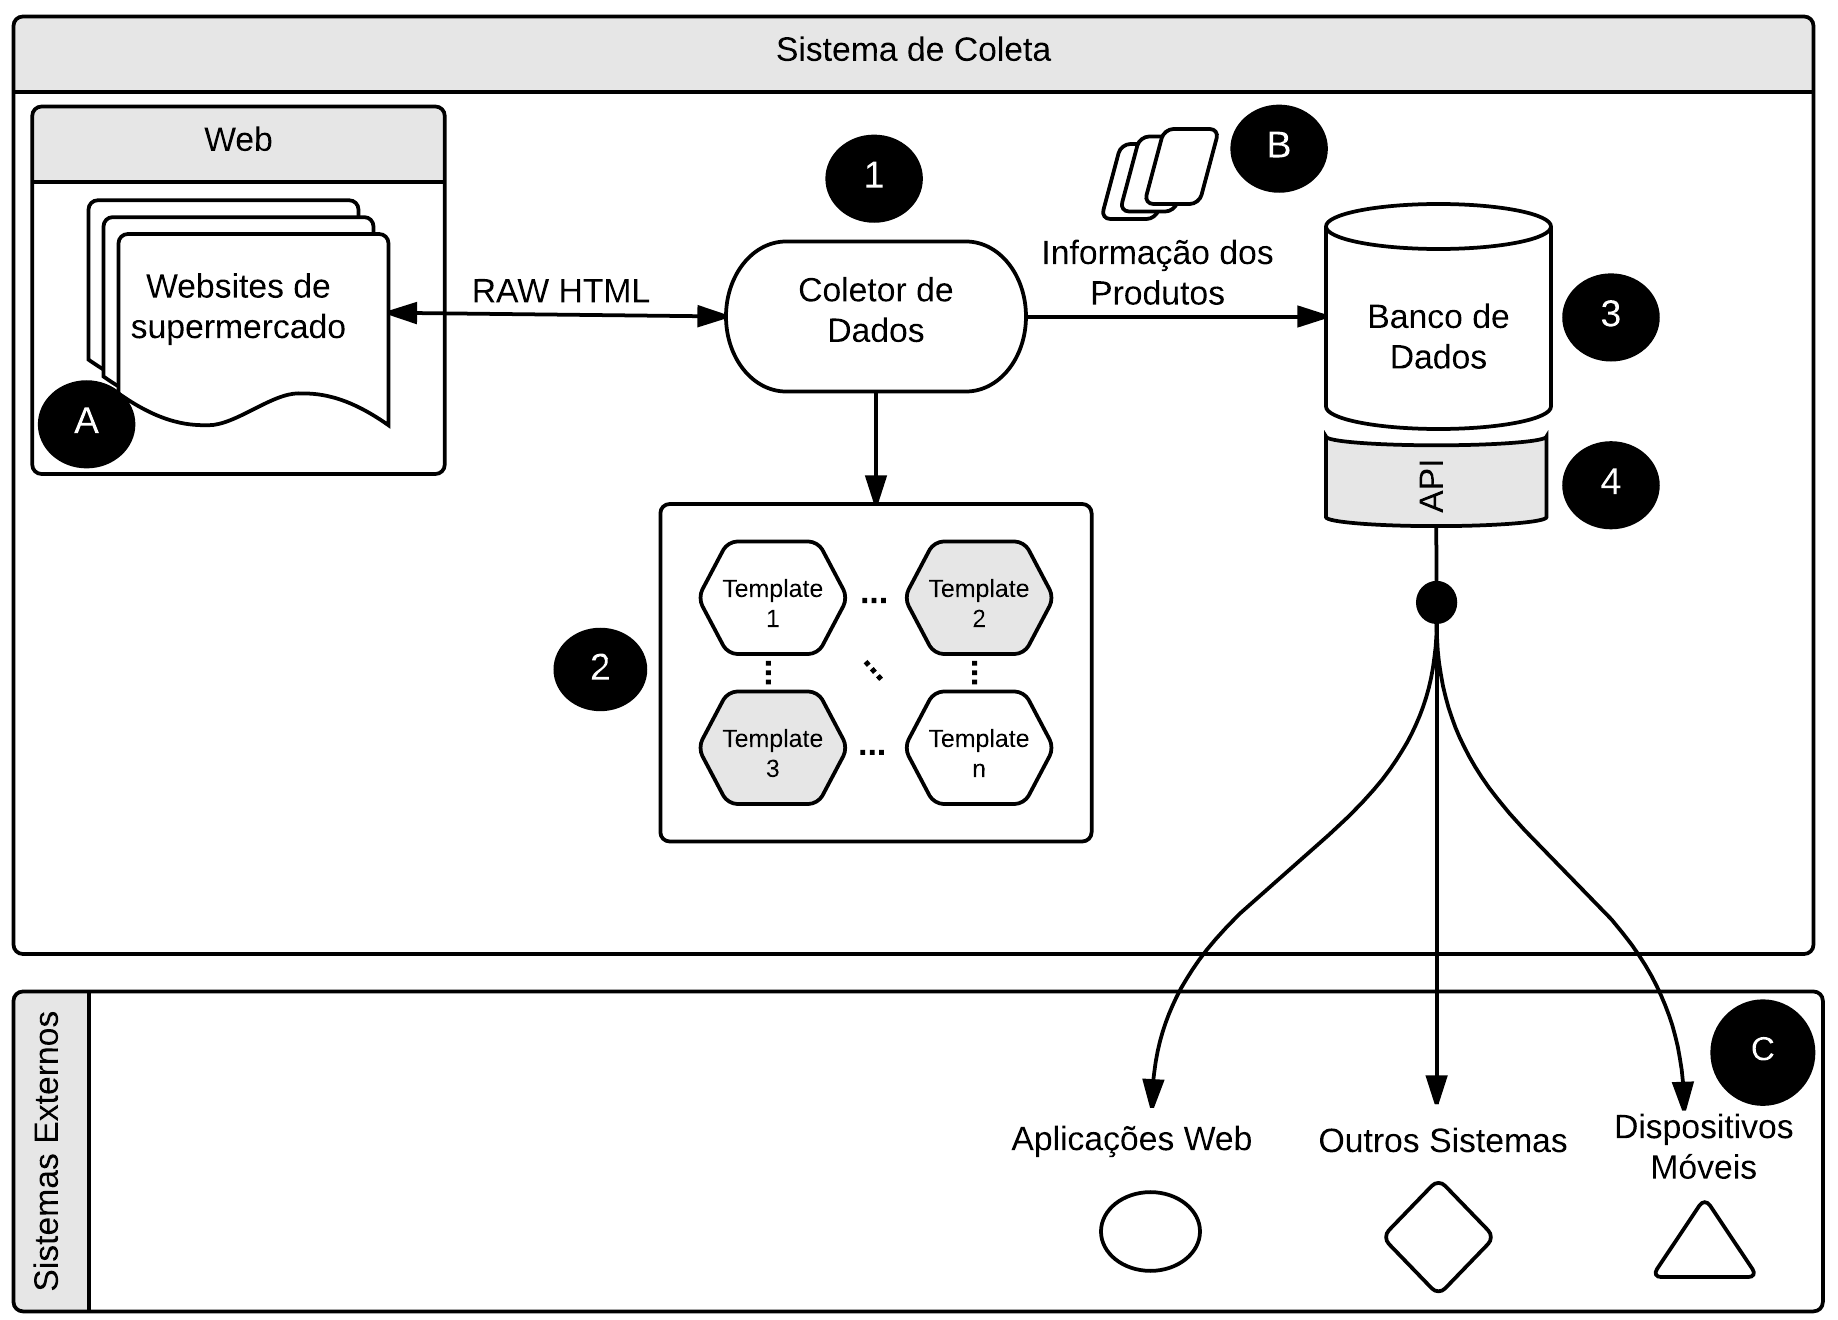
\includegraphics[width=\textwidth]{WebScraping}
  \caption[Figura Simples]{Arquitetura do Sistema de Coleta e Disponibilização dos Dados}
  \label{fig:01}
\end{figure}

Através de um coletor é possível arquiteturar e executar de forma lógica e escalável todo esse processo. Para que um coletor seja funcional é necessário que o mesmo seja capaz de interagir com páginas da Web, extrair a informação de interesse e estruturar e armazenar os dados para futuras consultas. Em geral, exemplos corriqueiros de coletores podem ser citados como os desenvolvidos pelo Google e Microsoft para atuar na procura por páginas da internet ou outros mais específicos para coleta de preços de produtos como os portais de agregadores como Bom de Faro, Buscapé dentre outros. Assim, como \citet{cavallo2010scraped}, o presente projeto de tese busca de forma inovadora para a economia brasileira, explorar preços coletados de sites de supermercados, farmácias, companhia de energia elétrica, lojas de varelo online, lojas de roupas e calçados, entre outros, e propõe o uso de um sistema de coleta como o apresentado a seguir. 

O sistema de coleta de preços está apresentado na Figura~\ref{fig:01}. O coletor recebe como entrada os templates dos sites que se deseja coletar e produz como resposta informações estruturadas com os atributos dos produtos. Para que o coletor seja capaz de realizar a tarefa de extração de informação, o mesmo deve apresentar os seguintes componentes: um componente centralizado capaz de ler instruções e aplicar regras para extração (1 - módulo coletor de dados); ter um conjunto de regras que descreva de forma não ambígua como realizar a coleta dos dados e os atributos de interesse (2 - templates dos webistes de supermercado, por exemplo); ter um banco de dados capaz de lidar com as características dos dados armazenados (3 - módulo de banco de dados); ter uma interface para facilitar o acesso aos dados por meio de outras aplicações ou sistemas web (4 - módulo de disponibilização da informação). Dessa forma, o coletor (1) é o centralizador do processo de coleta de dados, fazendo a interação com os templates (2), os webistes (A) e o módulo de banco de dados (3). Em resumo, o coletor através de um algoritmo inicia o processo de coleta carregando em uma lista os templates de coleta dos websites (2) e em seguida através de um processo iterativo visita o website, coleta os documentos de interesse e realiza a extração das informações indicadas pelo template. Ao final da coleta os dados são estruturados em um formato de documento denominado JSON e armazena-os em um banco de dados NoSQL adequado a essa estrutura de dados. O processo se repete para cada template até que todos os templates sejam avaliados. O algoritmo que descreve esse processo é apresentando em Algoritmo 1. Por fim, além da coleta em si, há um módulo para disponibilizar o acesso a informação coletada. Esse módulo (4) é responsável por permitir de forma segura e racional o uso dos dados coletados por diferentes sistemas e aplicações web existentes (C).

Segundo \citet{cavallo2010scraped}, preços coletados da internet possuem duas desvantagens: Primeiro, percentual menor de empresas disponibiliza seus produtos e preços na internet em comparação com as lojas físicas. Tal limitação pode ser minimizada ao longo do tempo com uma maior oferta de produtos e serviços na internet. Segundo, os preços coletados da internet não incluem informações sobre as quantidades vendidas o que impede de obter market share e estimativas de elasticidade.

Avaliações futuras precisarão ser feitas de forma que seja capaz explorar se os preços online e off-line se comportam similarmente. Preocupado com tal validação, \citet{cavallo2010scraped} fez pesquisa de preços nas lojas físicas dos supermercados utilizados para coleta de dados da internet. Desta forma, o autor examinou se os preços dos produtos nas lojas físicas eram similares aos preços nos sites. Uma importante característica é que um alto percentual de produtos vendidos nas lojas físicas também era comercializado nos sites em todos os países. O autor comparou os preços tanto em termo de nível quanto em tamanho e intervalo de tempo de alterações nos preços. Tal comportamento é muito importante para a avaliação de rigidez nos preços. Para tanto, o autor criou uma série de mudança de preços para cada produto que recebe valor 1 se o preço aumentou, 0 se o preço permaneceu constante e -1, caso contrário.  Assim, foi possível avaliar se os preços dos produtos nas lojas físicas são semelhantes em nível e em direção de mudança para cada produto e supermercado dos países avaliados por \citet{cavallo2010scraped}.

Não obstante, \citet{cavallo2010scraped} apresenta algumas vantagens dos preços coletados da internet que os fazem uma fonte única de informação para análise de rigidez nos preços. Primeiro, pode-se obter preços diários para os produtos e serviços e por conseguinte, reduzir medidas de erro em relação à frequência de cálculo da inflação, analisar promoções de produtos, controles e sincronização nos preços. Segundo, os dados estão disponíveis para vários países, com maior facilidade de acesso e possibilidade de comparação entre países. Terceiro, existem informações detalhadas sobre cada produto e não há substituições forçada de itens como ocorre em estatísticas oficiais de inflação. Por fim, preços coletados da internet estão viáveis em tempo real, sem qualquer atraso para acessá-los. Isto pode ser usado para providenciar estimativas de rigidez nos preços em tempo real.
  
\section*{ÍNDICE DE PREÇOS ONLINE}
  
Para calcular o índice de preços online que será comparado com o Índice Nacional de Preços ao Consumidor Amplo (IPCA) e Índice Nacional de Preços ao Consumidor (INPC) divulgados pelo Instituto Brasileiro de Geografia e Estatística (IBGE), utilizaremos a abordagem proposta por \citet{cavallo2010scraped}.
  
Assim, o índice de preços usa a combinação de dados online e as estruturas de ponderação oficiais do IBGE para as categorias da “cesta de mercadorias”\footnote[1]{Segundo o \citet{ibgemetodos} os índices constituem uma medida síntese de movimento de preços de um conjunto de bens e serviços, chamado “cesta de mercadorias”, representativo de um determinado grupo populacional, em certo período de tempo} de cada índice de inflação. Maiores detalhes sobre a metodologia de coleta e cálculo do IPCA e INPC podem ser obtidas no~\ref{ap1}. Dados diários serão utilizados para construir o índice de preços online o que é útil para observar padrões de curto prazo nos dados que ajudam a validar as informações online. 
  
O índice de preço online será calculado utilizando os preços de todos os produtos disponíveis para compra em cada site. Isto implica que a cesta de bens muda dinamicamente ao longo do tempo podendo um produto aparecer ou desaparecer da cesta a qualquer momento devido à disponibilidade ou indisponibilidade no site. Além disso, o número de preços por produto tende a ser muito maior o que os coletados usualmente pelos órgãos governamentais. 
Para construir o índice, mudanças de preço são calculadas em nível de produto, então as médias dentro das categorias usando média geométrica ponderada e finalmente agregado entre categorias com uma média aritmética ponderada. Em particular, o primeiro passo é obter a média geométrica ponderada das mudanças nos preços na categoria $j$ para cada dia $t$:

\begin{equation}\label{eq1}
R_{t,t-1}^{j}=\prod_{i}\left(\frac{p_{t}^{t}}{p_{t-1}^{i}}\right)^{\nicefrac{1}{n_{j,t}}}
\end{equation}

\noindent onde $p_{t}^{i}$ é o preço do bem $i$ no tempo $t$, $n_{j,t}$ é o número de produtos na categoria $j$ que estão presentes na amostra neste dia. 

O segundo passo é computar o índice em nível de categoria em $t$:

\begin{equation}\label{eq2}
I_{t}^{j}=R_{1,0}^{j}\ast{R}_{2,1}^{j}\ast{...}\ast{R}_{t,t-1}^{j}
\end{equation}

Finalmente, o índice de preços no tempo $t$ é a média aritmética ponderada de todos os índices das categorias:

\begin{equation}\label{eq3}
IPO_{t}=\sum_{j}{\frac{w_{j}}{w}I_{t}^{j}} 
\end{equation}

\noindent onde $w^{j}$ é o peso oficial utilizado pelo IBGE para tal categoria e $W$ a soma de todos os pesos incluídos na amostra.

A classificação de produtos e pesos de categorias é uma das partes mais complexas deste processo. Nos dados originais, cada produto é atrelado à um endereço de web (URL) que corresponde à página onde o produto é localizado. 

\section*{RIGIDEZ DE PREÇOS}

 Diversas estatísticas poderão ser utilizadas para a análise da rigidez de preços coletados da internet, como por exemplo: frequência de produtos com alterações diarias e frequências de alta e baixa em relação ao total de alterações nos preços em um dia. Assim, teremos um parâmetro que reflete a probabilidade incondicional de mudança no preço de uma firma ao longo de um dado período de tempo. Porém, a análise da frequência apresenta uma visão parcial do comportamento dos preços e faz-se necessário avaliar o tamanho da mudança dos preços por meio do valor absoluto da alteração no preço de um determinado produto (tambéma o tamanho das mudanças positivas e negativas) e avaliação da sua distribuição de probabilidade. Desta forma, poder-se-a comparar o comportamento da inflação em determinadas regiões, municípios e estados em relação ao tamanho da mudança nos preços nestes locais. 
 
\citet{cavallo2010scraped} encontrou uma característica bimodal na distribuição do tamanho das alterações nos preços e uma forte queda da densidade das alterações próximo a 0\% em alguns países, o que é consistente com os modelos de custo de menu que mudanças muito pequenas não são ótimas na presença de custo de ajuste. Outro tipo de análise é a avaliação da assimetria na densidade das alterações que pode refletir maior quantidade de preços crescendo que diminuíndo. 
 
\subsection*{Análise de Sobrevida}

A análse de frequência ajudará na avaliação da rigidez de preços, mas ela sugere que a probabilidade de um preço se alterar é independente do tempo que uma mudança ocorre em relação à última alteração no preço. Ainda, a taxa de risco do preço se alterar é constante ao longo do tempo durante todo o período amostral. Embora esse método seja simples e efetivo para a comparação do grau de rigidez entre setores, regiões, cidades e países, um importante ponto reside sobre a forma da função risco. 

Para avaliar a função risco utilizaremos a Análise de Sobrevida assim como \citet{cavallo2010scraped}. Conforme \citet{colosimo2006analise}, em análise de sobrevivência, a variável resposta é, geralmente, o tempo até a ocorrência de um evento de interesse. Tal tempo é comumente conhecido como tempo de falha. Em medicina é comum o uso do método para a avaliação do tempo até a morte, transplante, doença, cura  entre outros. No contexto de preços, estamos interessados no tempo até o ajuste do preço. Assim, tanto o aparecimento do risco e o evento de falha ocorrem quando uma firma muda seus preços.  

A principal característica de dados de sobrevivência é a presença de censura que é a observação parcial da resposta. Isto se refere a situações em que por alguma razão, o acompanhamento do preço foi interrompido, seja porque a firma não vende mais um produto ou este não é produzido. A variável aleatória não-negativa $T$, usualmente contínua, que representa o tempo de falha, é geralmente especificada em análise de sobrevivência pela sua função de sobrevivência ou pela função de risco (tempo de falha). Estas duas funções são extensivamente usadas na análise de dados de sobrevivência. 

Segundo \citet{colosimo2006analise}, a função de sobrevivência é definida como a probabilidade de uma observação não falhar até um certo tempo $t$, ou seja, a probabilidade de uma observação sobreviver (preço não se alterar) ao tempo $t$. Por outro lado, se $T$ é a variável aleatória que mede a duração do preço, com função densidade $f\left(t\right)$ e densidade acumulada $F\left(t\right)$, o risco $h\left(t\right)$ é a probabilidade limite de que a mudança no preço ocorra em $t$, condicional ao preço não se alterar até este momento. 

\begin{equation}\label{eq4}
h\left(t\right)=\lim_{\Delta t\rightarrow 0}{\frac{Pr\left(t<T<t+\Delta t|t<T\right)}{\Delta t}=\frac{f\left(t\right)}{1-F\left(t\right)}} 
\end{equation}

Esta função risco mede o risco instantâneo de um preço se alterar, condicionado à sobrevida. Podemos adicionar todas as taxas de risco ao longo do tempo e obter o risco total de um preço alterar acumulado até o tempo $t$. Isto é representado pelo função risco acumulado, $H(t)$:

\begin{equation}\label{eq5}
H\left(t\right)=\int_{0}^{t}{h\left(u\right)du=-\ln{\left(1-F\left(t\right)\right)}} 
\end{equation}

$H(t)$ é um aumento, função ilimitada de $t$, que acumula a probabilidade condicional do preço mudar ao longo do tempo. No contexto de repetidas "falhas" (preço se alterar), ela pode ser interpretada com o número esperado de ajustamento nos preços de $0$ à $t$. O risco acumulado recebe grande atenção na Análise de Sobrevida porque ele é mais fácil de estimar do que a função risco sózinha. 

Para estimar $H(t)$ e $h(t)$ empiricamente, usaremos conforme \citet{cavallo2010scraped} uma abordagem não paramétrica dada por Nelson (1972) e Aalen (1978), que não requer hipóteses de distribuição de probabilidade. Métodos semi-paramétricos como o modelo Cox podem ser utilizados futuramente uma vez que permitem a incorporação de variáveis explicativas e a consideração da heterogeneidade não observável em nível de categoria de preços. Uma estimativa simples da função risco acumulado, $H(t)$, é dado por:

\begin{equation}\label{eq6}
\hat{H}\left(t\right)=\sum_{j|{t}_{j}\le t}{\frac{{c}_{j}}{{n}_{j}}} 
\end{equation}

\noindent onde ${c}_{j}$ é o número de preços que mudaram em ${t}_{j}$ e ${n}_{j}$ é o número de preços sob risco em ${t}_{j}$, ou seja, os preços que não alteraram e não foram censurados até o instante imediatamente anterior a $t_{j}$. O passo incremental $\frac{{c}_{j}}{{n}_{j}}$ é uma estimativa para a probabilidade do preço mudar em ${t}_{j}$, levando em consideração apenas aqueles preços que sobreviveram até este ponto no tempo. 

Para obter a função risco suavizada $\hat{h}\left(t\right)$, pode-se usar a seguinte equação:

\begin{equation}\label{eq7}
\hat{h}\left(t \right)=\frac{1}{b}\sum_{j\epsilon D}{K}\left(\frac{t-{t}_{j}}{b}\right)\Delta \hat {H}\left({t}_{j}\right) 
\end{equation}

\noindent onde $K$ é um kernel com densidade simétrica, $b$ é a \emph{bandwidth} de suavização e $D$ é o conjunto de vezes com mudança de preços. 

% \section*{CRONOGRAMA}
% 
% O começo do programa de doutorado se deu no início de 2012 e pretende-se acabá-lo em tempo regular, isto é, em março de 2016. Abaixo, segue o cronograma com as atividades previstas para cada trimestre.
% 
% \begin{table}[h]
% \begin{tabular}{llllll}
% \hline
% \multicolumn{1}{c}{\textbf{Atividades}}             & 1º Trimestre 2015     & 2º Trimestre 2015     & 3º Trimestre 2015     & 4º Trimestre 2015     & 1º Trimestre 2016     \\ \hline
% Pesquisa Bibliográfica                              & \multicolumn{1}{c}{X} & \multicolumn{1}{c}{X} &                       &                       &                       \\
% Mapeamento de sites                                 & \multicolumn{1}{c}{X} &                       &                       &                       &                       \\
% Implementação do sistema de coleta                  & \multicolumn{1}{c}{X} &                       &                       &                       &                       \\
% Criação dos Índices de Inflação                     &                       & \multicolumn{1}{c}{X} & \multicolumn{1}{c}{}  & \multicolumn{1}{c}{}  &                       \\
% Análise de Rigidez                                  &                       &                       & \multicolumn{1}{c}{X} & \multicolumn{1}{c}{}  &                       \\
% Avaliação dos Determinantes da Inflação nas Regiões &                       &                       &                       & \multicolumn{1}{c}{X} &                       \\
% Redação Final da Tese                               &                       &                       &                       & \multicolumn{1}{c}{X} & \multicolumn{1}{c}{X} \\
% Entrega da Tese para Defesa                         &                       &                       &                       &                       & \multicolumn{1}{c}{X} \\ \hline
% \end{tabular}
% \end{table}
% 

\subsection*{Modelo Logit de probabilidade dos preços alterarem}

A metodologia descrita nesta seção é baseada sobre \citet{aucremanne2005time} que usaram uma abordagem de dados em painel para encontrar os fatores determinantes da probabilidade de um preço se alterar na Bélgica. Abordagem similar também foi usada por \citet{lunnemann2005consumer} para \citet{baumgartner2005frequently} para a Austria e \citet{baudry2004price} para a França.

Para modelar a probabilidade de um preço mudar será preciso focar sobre os eventos de mudança nos preços enquanto ignoramos o tamanho da mudança nos preços. Assim, defina $Y_{jkt}$ como uma variável binária:

\begin{equation}\label{eq8}
Y_{jkt} =\begin{cases}1 &  P_{jkt} \neq P_{jk,t-1}\\0 & P_{jkt} = P_{jk,t-1}\end{cases}
\end{equation}

\noindent onde ${Y}_{jkt}$ indica se o preço do produto $j$ vendido pela firma $k$ foi alterado no começo do período $t$, e ${P}_{jk,t-1}$ é o preço do produto $j$ vendido pela firma $k$ no período $t$. 

A escolha das variáveis explicativas para o modelo é depende sobre as hipóteses sobre o mecanismo de formação de preços subjacente. Se assumimos que os definidores de preço aplicam a regra de precificação de \citet{calvo1983staggered}, então a probabilidade de ajuste dos preços não depende do preço decorrido desde a última alteração no preço ou sobre o estado da economia e a única variável explicativa será uma constante. Neste caso, o modelo logit de probabilidade da firma $k$ alterar o preço do produto $j$ no começo do período $t$ é a seguinte:

\begin{equation}\label{eq9}
Pr\left( { Y }_{ jkt }=1 \right) =\frac { exp\left( { \beta  }_{ 0 } \right)  }{ 1+exp\left( { \beta  }_{ 0 } \right)  } 
\end{equation}

Sobre a hipótese de uma regra de precificação conforme Calvo, a probabilidade do preço alterar é descrita apenas por ${ \beta  }_{ 0 }$. Quanto maior for ${ \beta  }_{ 0 }$ menos rígidos são os preços. A equação~\ref{eq9} pode ser transformada para incluir também os elementos do modelo de \citet{taylor1980aggregate}, que assume que as firmas ajustam seus preços depois de um número de períodos fixo desde a última mudança. Isto é feito afirmando que o truncamento ocorre depois de um número fixo de períodos.

Se for assumido uma regra de precificação, então, seguindo \citet{cecchetti1986frequency}, a firma $k$ mudará o preço do produto $j$ apenas se a diferença entre o preço desejado $P_{jkt}^{*}$ e o preço atual $P_{jkt}$ excede uma constante limiar $h_{jk}^{*}$ (especifica para cada produto e firma):

\begin{equation}\label{eq10}
Pr\left( { Y }_{ jkt }=1 \right) =Pr\left( \ln { \left( \frac { { P }_{ jkt }^{ * } }{ { P }_{ jkt } }  \right) \ge { h }_{ jk }^{ * } }  \right) 
\end{equation}

De acordo com \citet{cecchetti1986frequency}, a probabilidade de que a diferença entre o preço atual e desejado exceder um certo limiar pode ser expressa em termos de variáveis exploratórias: inflação acumulada até a última alteração do preço, tempo decorrido até a última alteração, tamanho da última alteração no preço e mudança acumulada na variável de demanda até o ajuste do preço anterior. Isso nos leva à seguinte representação logit do modelo de precificação estado-dependente:

\begin{equation}\label{eq11}
Pr\left( { Y }_{ jkt }=1 \right) =\frac { exp\left( { \beta  }_{ 0 }+\sum _{ i=1 }^{ N }{ { \beta  }_{ i }{ X }_{ i,jkt } }  \right)  }{ 1+exp\left( { \beta  }_{ 0 }+\sum _{ i=1 }^{ N }{ { \beta  }_{ i }{ X }_{ i,jkt } }  \right)  } 
\end{equation}

\noindent onde ${ X }_{ i,jkt }$ denota uma variável exógena da listadas anteriormente.

A equação~\ref{eq11} pode ser vista como uma extensão da equação~\ref{eq9}. Contudo, ela permite testar se todos os formadores de preços na economia são tempo-dependentes. Obviamente, se $\beta_{1},...,\beta_{N}$ não são significativamente diferentes de 0, podemos concluir que todas as firmas seguem um modelo de precificação de Calvo. Por outro lado, estimativas significantes para qualquer $\beta_{1},...,\beta_{N}$ poderia ser interpretada como uma rejeição ao modelo de Calvo. \citet{aucremanne2005time} argumentam que as estimativas de $\beta_{1},...,\beta_{N}$ capturam tanto o impacto das variáveis sobre a probabilidade do preço alterar e a participação deste particular comportamento. Portanto, a rejeição do modelo de Calvo não significará que não existem formadores de preço que seguem esta regra na economia. Ao contrário, indicará que existe uma participação significativa de firmas seguindo o modelo de precificação estado-dependente.

\subsection*{Determinantes para a probabilidade do preço alterar}

A seguir possíveis variáveis a serem utilizadas no modelo logit para investigar os fatores que afetam a frequência com que os preços aos consumidor se alteram:

\begin{enumerate}
  \item Inflação: sobre as hipóteses dos modelos de precificação estado-dependentes de acordo com \citet{cecchetti1986frequency}, inflação total acumulada até a última alteração no preço estaria entre as variáveis. Maior a inflação acumulada está associado com duração curta entre mudanças nos preços. Em pesquisas empiricas, a abordagem para mensurar a inflação acumulada diverge. \citet{aucremanne2005time} alteraram a especificação de \citet{cecchetti1986frequency} através da substituição da inflação acumulada pela inflação acumulada mensurada ao nível setorial, enquanto as mudanças na inflação total foram consideradas por um conjunto de variáveis \emph{dummy}. A mesma abordagem foi usada em \citet{baumgartner2005frequently}.
  \item Tempo desde a última alteração: O tempo passado até o último ajuste de preço é uma importante variável explicativa tanto em modelos estado-dependentes e modelos tempo-dependentes. Por um lado, usando o modelo de limite-alvo \citet{cecchetti1986frequency} provaram, tanto teóricamente e empiricamente, que quanto maior o período desde a última alteração, maior a probabilidade de observar outra alteração no preço. Não obstante, o modelo de Taylor assume o truncamento de um preço depois de um período fixo no tempo. Um coeficiente positivo e estatisticamente significante indicará que uma participação significante das firmas segue uma regra de precificação tempo-dependente até alterar os preços depois de um certo número de meses, dias ou semanas.
  \item Tamanho da alteração anterior: \citet{cecchetti1986frequency} argumentam que o tamanho da alteração anterior nos preços pode conter informações sobre a próxima mudança no preço. Um ajuste passado grande poderia indicar que o limite para alterar os preços é alto e as firmas estão focadas a mudar os preços em frequência menor, embora que por montantes maiores. Da mesma forma, um ajuste passado pequeno poderia indicar que o limite é baixo e os preços podem mudar mais frequentemente. 
  \item Variável de demanda: O modelo teórico e empírico de \citet{cecchetti1986frequency} mostrou a importância do fator demanda (representada pelo montante de vendas da indústria) para a frequência das alterações nos preços. De acordo com seu estudo para preços de revistas, o efeito da demanda é positivo e estatisticamente significante. Assim, será preciso definir uma variável que represente a demanda dos produtos, pois na coleta de dados da internet não é possível mensurar a demanda sobre os itens disponíveis e apenas os preços.
  \item Atratividade dos preços: A frequência com que os preços se alteram pode ser afedata por efeitos psicológicos e estratégias de marketing. Um dos efeitos que é usualmente incluído nos modelos logit de mudanças de preços é o efeito de um preço atrativo. Como em \citet{aucremanne2005time}, pode-se definir a atratividade dos preços como um preço finalizando com os dígitos 9, 5 ou 0. A variável pode ser inserida no modelo por meio de \emph{dummies}.
  \item Efeito Sazonal e anual: O ajuste nos preços pode mostrar padrões sazonais que serão capturados por variáveis \emph{dummies} que dependerão da periodicidade dos preços coletados. Portanto, essas variáveis podem ser interpretadas como o efeito da omissão de condições macroeconômicas como, por exemplo, fatores de oferta e demanda. 
  \item Variáveis setoriais: Finalmente, os mecanismos de formação dos preços podem diferir entre firmas e estabelecimentos por setor de atuação. Este efeito pode ser capturado por um conjunto de variáveis que incluirão \emph{dummies} para os principais setores da economia.
\end{enumerate}

Assim, a representação do modelo logit considerando a abordagem de precificação estado-dependente da equação~\ref{eq11} é agora estendido para permitir efeitos aleatórios $u_{jk}$ que são específicos para todos os pares de produto-firmas:

\begin{equation}\label{eq12}
Pr\left( { Y }_{ jkt }=1 \right) =\frac { exp\left( { X }_{ jkt }\beta +{ u }_{ jk }+{ \varepsilon  }_{ jkt } \right)  }{ 1+exp\left( { X }_{ jkt }\beta +{ u }_{ jk }+{ \varepsilon  }_{ jkt } \right)  } 
\end{equation}

\noindent onde ${ X }_{ jkt }$ é um vetor linha de variáveis exógenas, $\beta$ é um vetor coluna dos coeficientes do modelo logit e ${ \varepsilon  }_{ jkt }$ é um termo de erro. Por fim, pode-se distinguir a variável $Y_{jkt}$ entre alterações em todos os preços ou excluir as promoções da análise. 



% \SweaveInput{cap4.Rnw}
% \SweaveInput{final.Rnw}

% Formato da bibliografia
\bibliographystyle{apalike}

% Arquivo .bib
\bibliography{projeto}

% Apêndice(s)
% \SweaveInput{apendice}
% \SweaveInput{apendice2}

% Fim do texto
\end{document}
